\documentclass[10pt,a4paper]{article}

\usepackage[colorlinks=true,urlcolor=blue,linkcolor=blue]{hyperref}
\usepackage[utf8]{inputenc}
\usepackage[T1]{fontenc}
\usepackage[french]{babel}
\usepackage{fancyvrb}
\usepackage{tikz}
\usepackage{pgf-umlsd}
\usepgflibrary{arrows}

\usepackage{float}
\usepackage{graphicx}

\title{Cahier des besoins - Reversi}
\author{Guillaume CHUPIN, Benoit FAGET, Alexis PICHON, Julien PILLEUX}

\begin {document}
\maketitle
\newpage
\tableofcontents
\newpage

\section{Introduction}

Notre projet consiste en l'élaboration d'un joueur de Reversi complet développé en suivant certaines règles afin de pouvoir être confronté à d'autre implémentations au cours d'un tournoi prévu qui confrontera notre programme à celui d'une seconde équipe de développement ayant reçu le même sujet.\\

Nous avons eu le choix entre utiliser le langage de programmation C ou le C++, nous avons décidé de prendre le C++. Notre programme appliquera les algorithmes les plus fréquents pour un joueur de Reversi et utilisera au mieux les bitboards. Un bitboard est une structure de données qui est très efficace pour encoder un plateau de jeu tel que celui du reversi, un bitboard est un ensemble de bit ou chaque bit correspond à une case du plateau et indique la présence ou l'absence d'une pièce, ainsi on devra utiliser deux bitboards, un pour la présence de pion blanc et un autre pour la présence de pion noir. L'interface utilisateur sera purement en mode texte dans un bash, on se concentrera plutôt sur le développement d'heuristiques propres au jeu. Le projet sera essentiellement dirigé vers l'utilisation de techniques d'exploration d'arbre classiques telles que Minimax-ab, Negamax, Negascout, MTD(f), Monte-Carlo Tree Search (MCTS), etc. Il nous reste à définir laquelle développer en première, et si nous aurons le temps d'en faire d'autres.

\section{Description et analyse de l'existant}

Le jeu de Reversi consiste en un jeu de pions opposant deux adversaires dont le but est de terminer avec le plus grand nombre de pions à la fin de la partie. La partie se termine lorsque plus aucun mouvement n'est possible pour chacun des deux joueurs. Le jeu commence avec quatre pions, deux par joueur, posé au centre d'un plateau de huit par huit (taille conventionnelle, mais il existe des variantes avec un plateau plus petit ou plus grand), comme sur la Fig \ref{fig:début_du_jeu}.
 \begin{figure}[H]    
    \centering
    \begin{BVerbatim}
       1 2 3 4 5 6 7 8
     A _ _ _ _ _ _ _ _
     B _ _ _ _ _ _ _ _
     C _ _ _ _ _ _ _ _
     D _ _ _ O X _ _ _
     E _ _ _ X O _ _ _
     F _ _ _ _ _ _ _ _
     G _ _ _ _ _ _ _ _
     H _ _ _ _ _ _ _ _
    \end{BVerbatim}
    \caption {Initialisation du jeu.\label{fig:début_du_jeu}}
    \end{figure}
Un joueur ne peut placer un pion que sur une case vide adjacente a un pion adverse et que si le pion ainsi posé permet la capture d'au moins un pion adverse. Pour capturer les pions adversaires, il faut que ceux-ci se retrouve entre un de vos pions déjà présent et celui que vous vous apprêtez à poser sur le plateau. La capture de pions peut s'effectuer dans les huit directions à la fois (voir Fig \ref{fig:aire_de_capture}).
 \begin{figure}[H]    
    \centering
\begin{tikzpicture}

  \node (x) {X};
  \node (r) at (0.8,0) {};
  \node (ru) at (0.63,0.63) {};
  \node (u) at (0,0.75) {};
  \node (lu) at (-0.63, 0.63) {};
  \node (l) at (-0.8, 0) {};
  \node (ld) at (-0.63, -0.63) {};
  \node (d) at (0, -0.75) {};
  \node (rd) at (0.63, -0.63) {};
  
  \draw[->] (x) -- (r);
  \draw[->] (x) -- (ru);
  \draw[->] (x) -- (u);
  \draw[->] (x) -- (lu);
  \draw[->] (x) -- (rd);
  \draw[->] (x) -- (d);
  \draw[->] (x) -- (ld);
  \draw[->] (x) -- (l);
  \end{tikzpicture}
    \caption {Aire de capture d'un pion.\label{fig:aire_de_capture}}
 \end{figure}
 \tikzstyle{block} = [rectangle, draw, text width=6em, text centered, rounded corners, minimum height=4em]
 
\subsection{Programmes}
Pour qu'un programme puisse savoir quel coup jouer, il faut qu'il calcule qu'elles peuvent être les réponses de son adversaire et ainsi se projeter quelques coups dans l'avenir. On stocke cela dans un arbre où les noeuds correspondent à l'état du jeu et les arcs sont les coups joués(voir Fig \ref{fig:exemple_arbre}).
  \begin{figure}[H]    
    \centering
 \begin{tikzpicture}
     
\node[block] (a) at (3,5){\begin{BVerbatim}
  1 2 3 4 5 6
A _ _ _ _ _ _
B _ _ _ _ _ _
C _ _ O X _ _
D _ _ X O _ _
E _ _ _ _ _ _
F _ _ _ _ _ _ 
\end{BVerbatim}
     };
 \node[block]  (b) at (-1,0) {\begin{BVerbatim}
  1 2 3 4 5 6
A _ _ _ _ _ _
B _ _ _ _ _ _
C _ X X X _ _
D _ _ X O _ _
E _ _ _ _ _ _
F _ _ _ _ _ _ 
\end{BVerbatim}
 };
  \node[block]  (c) at (2,0) {\begin{BVerbatim}
  1 2 3 4 5 6
A _ _ _ _ _ _
B _ _ X _ _ _
C _ _ X X _ _
D _ _ X O _ _
E _ _ _ _ _ _
F _ _ _ _ _ _ 
\end{BVerbatim}
  };
    \node[block]  (d) at (5,0) {\begin{BVerbatim}
  1 2 3 4 5 6
A _ _ _ _ _ _
B _ _ _ _ _ _
C _ _ O X _ _
D _ _ X X X _
E _ _ _ _ _ _
F _ _ _ _ _ _ 
\end{BVerbatim}
    };
 \node[block]  (e) at (8,0) {\begin{BVerbatim}
  1 2 3 4 5 6
A _ _ _ _ _ _
B _ _ _ _ _ _
C _ _ O X _ _
D _ _ X X _ _
E _ _ _ X _ _
F _ _ _ _ _ _
\end{BVerbatim}
    };
      
  \draw[->] (a) -- node [text width=2em,midway,above] {c2} (b);
  \draw[->] (a) -- node [text width=2em,midway,above] {b3} (c);
  \draw[->] (a) -- node [text width=3em,midway,above] {d5} (d);
  \draw[->] (a) -- node [text width=4em,midway,above] {e4}(e);
 \end{tikzpicture}
     \caption {Exemple d'arbre.\label{fig:exemple_arbre} }
 \end{figure}
  Un programme qui ainsi pourrait prévoir tous les coups possible pourrait facilement savoir quel coup jouer, mais de part le nombre exponentiel de coup possible il n'est pas envisageable de le faire dans un temps restreint, il faut donc trouver un moyen d'obtenir de bon résultat sans explorer entièrement l'arbre de recherche des coups possibles.\newline
  La majorité, si ce n'est tout, les algorithmes utilisent la méthode minimax pour trouver le meilleur coup à jouer dans l'arbre. Minimax ce base sur le fait que l'ennemi répondra de la manière la plus avantageuse pour lui, donc on doit choisir le meilleur coup à jouer en sachant que l'ennemi fera de même. Afin, de connaître les chances de gagner pour le joueur avec un certain coup, minimax utilise une fonction d'évaluation.

 Cette fonction d'évaluation se base principalement sur deux principes du jeu.
  \begin{itemize}
  \item \textbf{Stabilité des pions}: Un pion est dit stable si l'ennemi n'a pas la possibilité de pouvoir le reprendre et ce pour le reste de la partie. Ainsi, les quatre coins du plateau de jeu sont des positions ou les pions seront stables. De plus, les pions adjacent de la même couleur obtiendrons également le statut stable. Par exemple dans la Figure \ref{fig:pion_stable}, tous les pions du plateau sont stable.
   \begin{figure}[H]    
    \centering
    \begin{BVerbatim}
       1 2 3 4 5 6
     A X _ _ _ _ X
     B X _ _ _ _ _
     C X _ _ _ _ _
     D X _ _ _ _ _
     E X _ _ _ X X
     F X _ _ _ X X 
    \end{BVerbatim}
    \caption {Exemple de pions stable.\label{fig:pion_stable}}
   \end{figure}

\item \textbf{Mobilité}: Avoir un grand choix de coup est assez important, car augmente les chances d'avoir de bon coup, tandis qu'avoir un faible nombre de coup nous entraînera inéluctablement vers de mauvaise décision, voir pire vers aucune décision possible et dans ce cas la défaite nous est quasiment assurée. Ainsi, l'idéal est d'avoir un grand choix de coups, tout en réduisant le nombre de coups de l'adversaire (et ainsi réduire ses possibilités de victoire).
  \newline
  De plus, faire le dernier coup, est assez avantageux, car permet de prendre des pions qui ne seront jamais repris, car la partie sera finie, ainsi il peut être intéressant si on n'a pas le coup final, d'essayer d'obtenir le dernier coup. Naturellement c'est le joueur blanc qui  a ce dernier coup, ainsi le joueur noir souhaitant obtenir le dernier coup devra faire passer un tour au joueur blanc.
  Cette notion de dernier coup, existe aussi avant la fin de la partie, en effet, sur le plateau il apparaîtra, vers la fin de la partie, différente zone ou cette technique de dernier pourra également être utilisé.
  Par exemple, dans la Figure \ref{fig:mobilité}, le joueur noir à la possibilité d'avoir un dernier coup local en g8, alors que s'il décidé de jouer en a2 il donnerais la possibilité au joueur blanc de faire un dernier coup local en a1.
  \begin{figure}[H]    
    \centering
    \begin{BVerbatim}
       1 2 3 4 5 6 
     A _ O O O _ _
     B _ X O X _ O
     C O X O X O O
     D O X X X X O
     E X X X O O O
     F O O O O _ O 
    \end{BVerbatim}
    \caption {Exemple du principe de mobilité.\label{fig:mobilité}}
  \end{figure}
    \end{itemize}
\subsubsection {Iago}
Dans les années 1980, un programme nommé Iago est développé. Il fut parmis les premiers programmes à démontrer qu'il était possible de créé un programme capable de battre le meilleur joueur humain.
Ce dernier, optimise la recherche du prochain coup en limitant la recherche à un certain nombre de coup dans le futur, déterminé par le temps alloué pour ledit coup.\newline

Il améliore également minimax en réduisant le nombre de noeuds évalué en n'explorant pas certains sous arbre dont peut déjà savoir qu'ils ne nous mèneront pas vers un meilleur résultat que les sous-arbres déjà exploré. Ainsi, l'ordre dans lequel les branches sont évaluées est importante, ainsi pour chaque recherche Iago organise ses noeuds dans l'ordre croissant.\newline

La fonction d'évaluation dont il hérite à été faite a la ``main'', en effet ils ont testé plusieurs variations, basé sur les principes vu précédemment, en les faisant s'affronter l'une contre l'autre et ont gardé la meilleure.



\subsubsection {Bill}
Peu après la création de Iago, le programme Bill est également créé et ce dernier bat Iago à chaque fois.
Il est assez similaire à Iago, mais combine les probabilités avec l'utilisation de Minimax, permettant de mieux simuler le comportement humain. Ainsi, un coup légal obtient une probabilité de 100\% tandis que les coups illégaux ont une valeur calculée. Ensuite, le programme pourra facilement savoir quel coup privilégier afin d'atteindre assurément une case du plateau. \newline

Un autre ajout, est de bornée la valeur de retour de Minimax ce qui permet d'exclure plus de branche, mais le risque reste que si la borne a été mal choisie la recherche retourne une valeur incorrect, mais pour parer cela il suffit de voir si la valeur retournée correspond à une des bornes est ainsi on sera que le résultat se situe en dehors de ces bornes.
\newline

Il utilise également une table de hashage pour stocker les meilleurs coups obtenus %%voir l'utilité de cette table%%
 et profite également du temps que son adversaire met à jouer pour la mettre à jour (alors que Iago se contentait d'attendre le coup de l'adversaire). 

\subsubsection {Logistello}
\newpage
\section{Besoins fonctionnels}
\label{sec:besoins_fonctionnels}

\subsection {Déroulement d'une partie}
\label{sec:deroulement_partie}

% Diagrammes de séquences
\begin{figure}[H]
  \centering
  \begin{sequencediagram}
    % Instances
    \newthread[blue]{user}{User} %[couleur]{nom 'variable'}{nom affichage}
    \newthread[green]{game}{Reversi} % [distance]
    \tikzstyle{inststyle}+=[bottom color=white, top color=white, rounded corners = 3mm]
    \newinst[4]{board}{Plateau} 

    % Instanciation Plateau
    \begin{messcall}{user}{./reversi}{game} % {source}{affichage}{destination}
      \begin{call}{game}{create\_board()}{board}{Display rules and board} % {source}{affichage}{destination}{retour}
      \end{call}
    \end{messcall}

    % Le joueur joue un coup
    \mess{user}{Play move}{game} % L'utilisateur choisi une case
    \begin{call}{game}{play\_move(String)}{board}{update\_display()} % Le jeu passe la chaîne correspondante au plateau
      \begin{call}{board}{check\_if\_valid()}{board}{valid OR not valid} % Le plateau vérifie la validité du mouvement.
      \end{call}
    \end{call}

    % La machine joue à son tour
    \begin{call}{game}{ia\_play\_move(String)}{board}{update\_display()} % Normalement pas besoin de vérifier (si on code ça bien).
    \end{call}

    % Le joueur décide de quitter
    \mess{user}{Enter q}{game}
    \mess{game}{Ask save}{user}
    \mess{user}{Type y}{game}
    \begin{call}{game}{save\_game()}{board}{}
    \end{call}
    \begin{call}{game}{quit()}{game}{}
    \end{call}
    
  \end{sequencediagram}
  \caption{Diagramme séquentiel de déroulement d'une partie.\label{fig:diagramme_partie}}
\end{figure}

\subsection{Listes des fonctionnalités}
\label{sec:fonctionnalites}

% Début nouvelle partie post TD1
\begin {itemize}
\item  L'entrée de l'utilisateur est insensible à la casse.
\item  L'utilisateur peut choisir un coup à jouer en entrant les coordonnées de la case où il désire jouer, par exemple il peut choisir la case \verb!a2!.
\item  L'utilisateur peut sauvegarder sa partie à tout moment en entrant le caractère 'q'. Le fichier de sortie de la sauvegarde est un fichier \verb!ASCII! contenant l'état actuel du plateau plus le tour du prochain joueur (voir Fig. \ref{fig:exemple_save}).
  \begin{figure}[H]    
    \centering
    \begin{BVerbatim}
      O
      _ _ _ _ _ _
      _ _ _ _ _ _
      _ _ X O _ _
      _ _ O X _ _
      _ _ _ _ _ _
      _ _ _ _ _ _ 
    \end{BVerbatim}
    \caption {Exemple de fichier de sauvegarde.\label{fig:exemple_save}}
    \end{figure}

\item  Le programme doit contenir un mode contest permettant de faire s'affronter deux intelligences artificielles. Ce mode de jeu prend en entrée un fichier de sauvegarde obtenu lorsque l'on quitte le programme.
\item  La taille du plateau de jeu est modifiable grâce grâce à une option de lancement. Lors du lancement -s ou --size suivit d'une valeur entre 1 et 5 ce qui fait varier la taille de la grille de 2 à 10 cases en ne prenant que des valeur paires (Voir Fig. \ref{fig:exemple_taille}). Par défaut, la grille affichée sera de dimension \verb!8x8!.
  \begin{figure}[H]    
    \centering
    \begin{BVerbatim}
        1 2 3 4 
      A _ _ _ _
      B _ _ _ _
      C _ _ _ _
      D _ _ _ _
      
    \end{BVerbatim}
    \caption {Exemple de grille générée avec l'option \textsc{-s2}.\label{fig:exemple_taille}}
  \end{figure}
\item  Il est possible de décider quel rôle donner à l'ia lors du lancement du programme.
  \begin{description}
  \item [-w, --white] Pour indiquer que l'ia jouera les pions blancs.
  \item [-b, --black] Pour indiquer que l'ia jouera les pions noirs.
  \item [-a, --all] Pour indiquer que l'ia jouera les deux camps.
  \end{description}
\item  La version du programme sera affichable avec l'option de lancement -V. 
\item  Le mode verbose de la partie sera activable au lancement du programme avec l'option -v. % Fleury a dit qu'il s'en battait les couilles du mode verbose hein.
\item  Une aide est disponible pour l'utilisateur grâce à l'option -h ou --help. Elle liste l'ensemble des options du programme ainsi que leur description.
\end{itemize}
% Fin nouvelle partie post TD1.

\newpage
\section{Besoins non fonctionnels}

\begin{itemize} 
\item Rapidité d'exécution : chaque coup doit être exécuté en moins d'une seconde.
\item Portabilité : le programme doit pouvoir s'exécuter sur toute machine de type Linux..
\item Confiance : les règles doivent être respectées et les fichiers de sauvegarde doivent suivre le format et la forme attendue (voir \ref{fig:exemple_save}).
\end{itemize}

\begin{figure}[H]
\centering
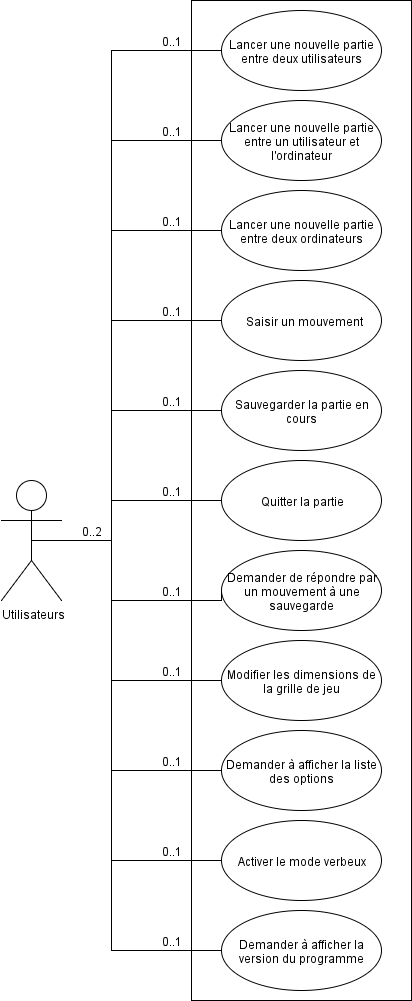
\includegraphics[scale=0.5]{images/use_case.png}
\label{use_case}
\caption{Diagramme de cas d'utilisation}
\end{figure}

\newpage
\section{Diagramme de Gantt}
\begin{center}
  \begin{tabular}{| l | c | c | c | c | c | c | c | c | c | c | c | c |}
    \hline
    Semaines     & 06 & 07 & 08 & 09 & 10 & 11 & 12 & 13 & 14 & 15  \\ \hline
    Game         & X  &    &    &    &    &    &    &    &    &     \\ \hline
    Board        & X  &    &    &    &    &    &    &    &    &     \\ \hline
    Input/Output &    & X  &    &    &    &    &    &    &    &     \\ \hline
    Player       &    & X  &    &    &    &    &    &    &    &     \\ \hline
    Game Tree    &    &    & X  & X  &    &    &    &    &    &     \\ \hline
    Heuristic    &    &    &    &    &  X & X  & X  & X  & X  & X   \\ \hline
  \end{tabular}
\end{center}

\section{Bibliographie}
\bibliographystyle{alpha}
\bibliography{reversi}
\nocite{*}

\end{document}
